% Notes:

\chapter{Background}

\section{Astronomy}

\subsection{Galaxy Morphologies}
Galaxy morphology refers to the physical shape of a galaxy.
Two main types of morphologies are elliptical (early-type) and spiral (late-type) galaxies.
In 1926, Edwin Hubble formulated developed an early classification scheme knows as the Hubble tuning fork diagram (Figure \ref{fig:tuning-fork}).
The diagram developed notation to refer to different traits found in morphologies.

\begin{figure}
    \centering
    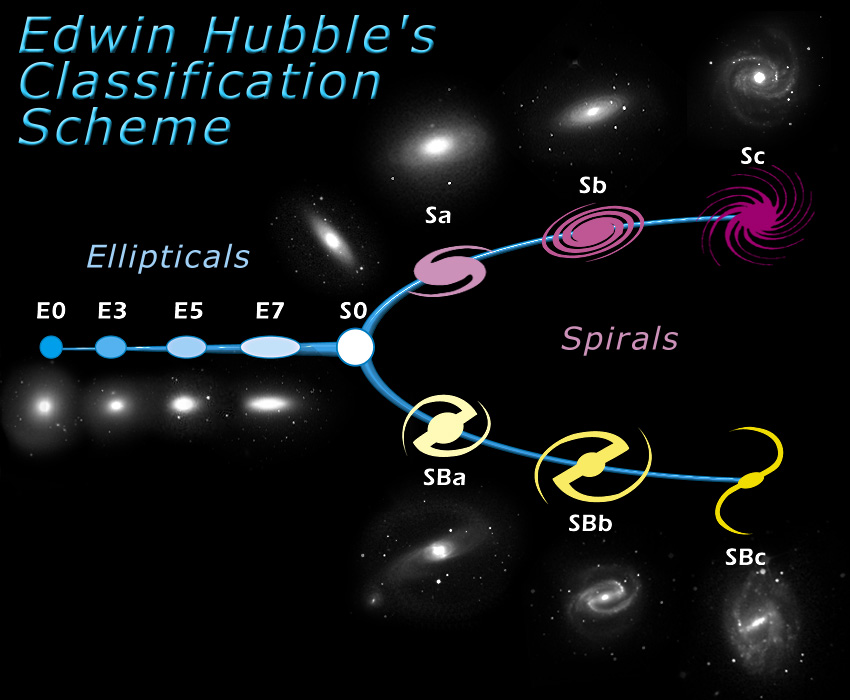
\includegraphics[width=0.8\linewidth]{tuning-fork}
    \caption[Hubble tuning fork diagram]{Edwin Hubble's tuning fork diagram via ESA/Hubble}
    \label{fig:tuning-fork}
\end{figure}

\section{Astronomical Data}
Modern professional astronomy has evolved to rely on solely digital data.
Telescopes use CCD (Charge-coupled device) cameras to produce digital images and spectrographs to measure spectra \citep{possel_beginners_2020}.
Spectrographs are prism-like devices which measure magnitude at different wavelengths \citep{noauthor_sdss_nodate}.
Apart from looking extensively at one celestial object, nowadays telescopes conduct full-blown sky surveys which document whole sections of the observable universe.
These surveys collect data into catalogues which combine other data points such as positional data and unique object identifiers \citep{possel_beginners_2020}.


\subsection{Photometric and Spectroscopic Data}
\textit{Photometric} and \textit{spectroscopic} are terms commonly used to distinguish between different types of astronomical data.
Photometric data is collected from the images themselves and is a measure for the brightness in a portion of an image, more commonly referred to as magnitude.
Data from the Sloan Digital Sky Survey (SDSS) includes multiple measures of photometry for a single image as an image is taken through five different coloured filters simultaneously \citep{noauthor_voyages_nodate}.
Spectroscopic data measures light at each wavelength. 
This allows the investigation of the chemical composition and physical properties of distant celestial objects \citep{i_appenzeller_immo_author_introduction_2013}.

\subsection{Sloan Digital Sky Survey}
The SDSS is a major survey founded with the intention of creating a detailed map of a large sector of the visible universe \citep{blanton_sloan_2017}.
The corresponding telescope found at Apache Point Observatory saw first light in 1998 and is considered to have achieved its goals since.
The SDSS comprises various sub surveys, each with different functions.
One example is the Baryon Oscillation Spectroscopic Survey (BOSS), focused on creating the largest three-dimensional map of galaxies to date.

\subsection{Visually Classified Data - Galaxy Zoo}
Visually classified datasets comprise data which has been manually analysed by experienced astronomers.
This process may involve assigning objects to their respective class, for example Stars, Galaxies and Quasars.
Another example would be to assign galaxies to their corresponding morphology class.

This leads us into the Galaxy Zoo project.
Galaxy Zoo is a large-scale crowdsourced project which uses an online tool to allow amateur astronomers to visually classify galaxies into morphological classes.
The two main phases of the project both involved classifying images from SDSS data releases,
with the second phase using a subset of the data from phase one, but the class count was significantly increased \citep{willett_galaxy_2013}\citep{lintott_galaxy_2008}.
Refer to appendix \ref{tab:sample-images} to view sample Galaxy Zoo 2 images.

\section{Data Science}

Modern Data Science refers to the extraction of information from data \citep{dhar_data_nodate}.
In the era of \textit{Big Data}, Data Science is crucial for gaining new and important knowledge.
Good data not only helps us explain the past but also provides predictive power, which is where Data Science comes into play.
One instance of this is Classification.

\subsection{Classification}
Classification problems involve taking labelled data and using it to train classifiers (Figure \ref{fig:classification}).
The classifiers are then used to classify data which is not labelled during the testing phase.
Classification makes for data which is structured, sortable, and easily analysed and understood \cite{suthaharan_machine_2015}.
In a context such as galaxy classification, this process can be applied to help understand the composition of the universe.

\subsection{Convolutional Neural Network}

\subsection{Key Performance Indicators}

\begin{figure}
    \centering
    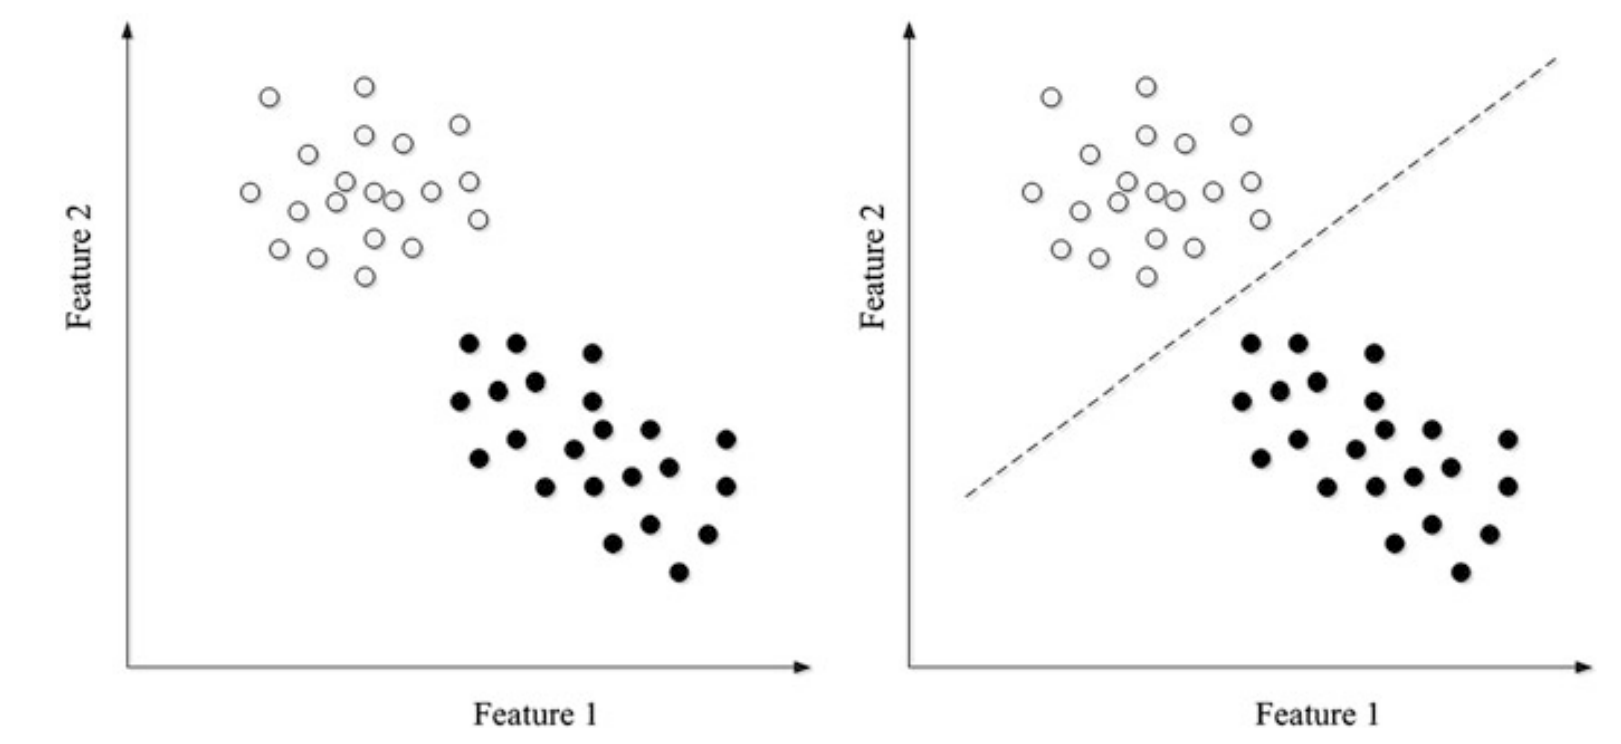
\includegraphics[width=0.9\linewidth]{classification}
    \caption[Classification scatter plot diagram]{Classification is defined \citep{suthaharan_machine_2015}}
    \label{fig:classification}
\end{figure}

\section{Pre-processing techniques}

\section{Data Augmentation}
Data Augmentation is crucial when working with imbalanced datasets to prevent overfitting.
Overfitting occurs when training a classifier with data that is of low quality and quantity.
This leads to classifiers which are biased to the training dataset and won't perform well with other samples.
Data augmentation prevents overfitting by creating copies of the existing sample to enhance the dataset \cite{lemley_smart_2017}.

\subsection{Generative Adversarial Networks}
